\chapter{\color{red} 数据库设计}
\section{数据库环境说明}
本系统的数据系统采用Oracle数据库系统,并基于关系数据库进行扩展\\
扩展部分结合非关系型数据库NoSQL实现\\
扩展原因为:\\
由于即时通讯中需要存储音频与视频,需要存储多媒体数据\\
多媒体数据与传统数据库数据有显著的不同,多媒体数据库有以下特点。\\
1)数据量巨大且媒体之间量的差异十分明显,而使得数据在库中的组织方法和存储方法复杂。\\
2)媒体种类的繁多使得数据处理变得非常复杂。\\
3)多媒体不仅改变了数据库的接口,使其声、图、文并茂,而且也改变了数据库的操纵形式,其中最重要的是查询机制和查询方法。媒体的复合、分散、时序性质及其形象化的特点,使得查询不再只是通过字符查询,查询的结果也不仅是一张表,而是多媒体的一组“表现”。接口的多媒体化将对查询提出更复杂、更友好的设计要求



\section{数据库的命名规则}
\begin{itemize}
    \item 1. 实体的命名方式为驼峰命名
    \item 2. 允许单词缩写,很长的单词可以采取辅音字母作为代表。例如tp表示第三方平台(third platform), pw表示password
    \item 3. 属性名采用小写命名的方式,可以通过下划线添加备注前缀
    \item 4. 字段不带类型前缀
    \item 5. 实体表名为单数
    \item 6. 关联表表名命名方法:将两个表名字的全称或缩写用下划线连接起来,对于两个实体间的多种关系,加入表示该关系的后缀
    \item 7. 字符数限制:20
\end{itemize}

\section{\color{red}逻辑设计}
\subsection{\color{red}实体与属性设计}
\begin{table}[htbp]
\centering
\caption{\color{red}实体设计} \label{tab:client-database}
\begin{tabular}{|c|c|c|c|c|}
    \hline
    实体 & 说明 & 属性 \\
    \hline
    用户 & 存储用户的信息和状态 & ID(主键),名字,email, 电话号码等 \\
    \hline
    团队 & 团队的信息 & 团队ID(主键), 队长ID, 队名等 \\
    \hline
    文件 & 传输的文件 & 文件ID(主键), 文件内容 \\
    \hline
    日历 & 所有用户的日历 & 用户ID(主键), 时间,内容 \\
    \hline 
    协作文档 & 存储在线协作文档 & 文档ID(主键), 文档内容 \\
    \hline
    issue & 存储团队中的issue & issueID(主键),issue内容, issue状态 \\
    \hline
\end{tabular}
\note{实体设计}
\end{table}

\subsection{\color{red}关系设计}
\newpage
\begin{table}[htbp]
\centering
\caption{\color{red}关系设计} \label{tab:client-database}
\begin{tabular}{|p{4em}|p{8em}|p{20em}|}
    \hline
    关系 & 说明 & 属性 \\
    \hline
    包含关系 & 团队包含用户 & ID(主键),名字,email, 电话号码等 \\
    \hline
    管理关系 & 团队管理文件 & 团队ID(主键), 用户ID(主键), 权限等 \\
    \hline 
    收发关系 & 用户收发文件 & 发送者ID(主键), 接收者ID(主键),文件ID(主键) ,发送时间\\
    \hline
    发布关系 & 团队发布日历 & 团队ID(主键), 用户ID(主键), 任务时间(主键),发布时间,任务内容等 \\
    \hline
    制定关系 & 用户制定日历 & . \\
    \hline 
    聊天关系 & 用户和用户聊天 & 发送者ID(主键), 接收者ID(主键),发送时间(主键),接受时间 \\
    \hline 
    好友关系 & 用户和用户是好友 & 用户一ID(主键), 用户二ID(主键) \\
    \hline
    调研关系 & 用户调研用户 & 用户一ID(主键), 用户二ID(主键),调研ID(主键)等\\
    \hline
    审批关系 & 用户和用户是好友 & 用户一ID(主键), 用户二ID(主键), 审批ID(主键)等\\
    \hline
\end{tabular}
\note{关系设计}
\end{table}
\subsection{\color{red} ER图}
        \begin{figure}[ht]
            \centering
            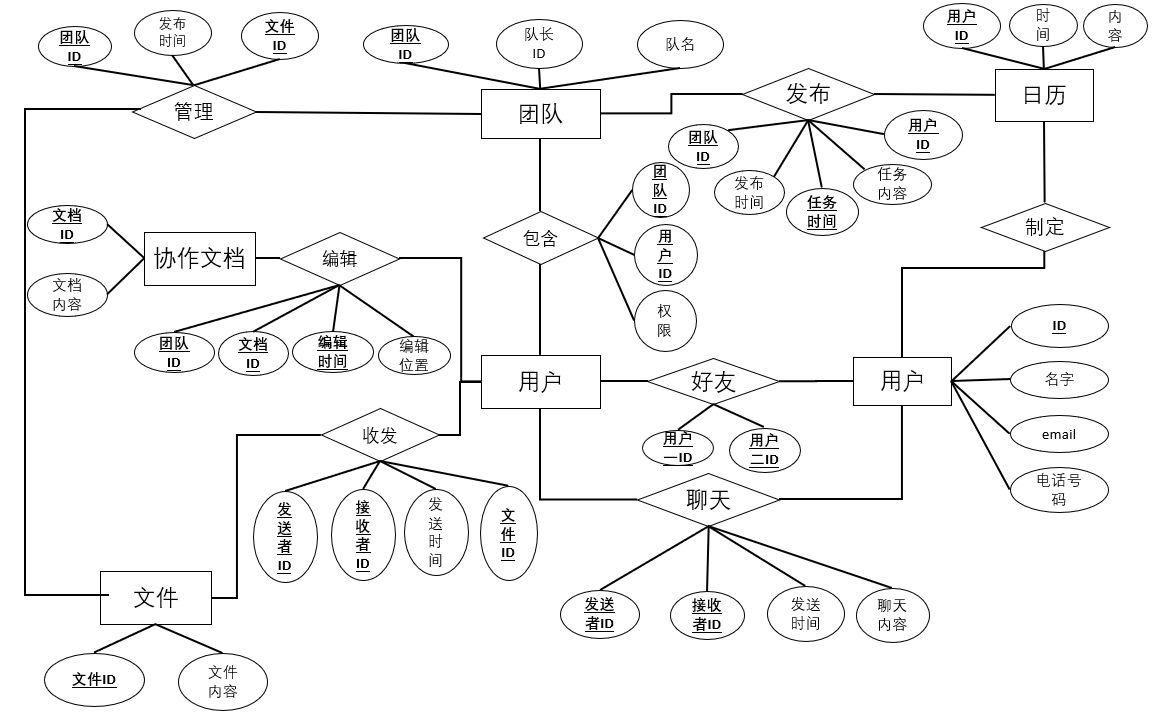
\includegraphics[scale =0.6]{数据库.png}\label{tab:classification}
            \caption{\color{red} 数据库逻辑图}\label{fig:noted-figure}
        \end{figure}
        \newpage


\section{\color{red} 物理设计}
\subsection{\color{red} 数据库产品}
\begin{itemize}
    \item 采用Oracle数据库和Hbase分布式数据库结合
    \item 采用Oracle集中数据库存储文件,用户信息
    \item 采用分布式数据库Hbase(NoSQL)存储聊天信息,多媒体信息
    \item 集中存储用户信息,文件有利于数据管理,分析,隐私保护
    \item 分布存储有利于系统性能提升,且可避免单点失效导致服务丢失
\end{itemize}


\subsection{\color{red} 实体属性、类型、精度}

\subsubsection{\color{red} 用户数据表设计}
\begin{table}[htbp]
\centering
{\color {red}
\caption{\color{red} 用户数据表User设计} \label{tab:client-database}
\begin{tabular}{|c|c|c|c|c|}
    \hline
    字段名 & 类型 & 大小 & 说明 & 备注 \\
    \hline
    id & char & 64 & 用户的唯一标识符 & 主键\\
    \hline
    name & char & 64 & 用户的名字 & · \\
    \hline
    email & char  & 64 & 用户的电子邮箱 & · \\
    \hline
    phone & char & 11 & 用户的联系电话 & · \\
    \hline
    tp\_id & char  & 64 & 第三方平台登陆账号 & · \\
    \hline
    tp\_pw & char & 64 & 第三方平台登陆密码 & · \\
    \hline
\end{tabular}
\note{\color{red}用户数据表User设计}
}
\end{table}
%========================================
\newpage
\subsubsection{团队数据表设计}
\begin{table}[htbp]
\centering
\caption{团队数据表Group设计} \label{tab:order-database}
\begin{tabular}{|c|c|c|c|c|}
    \hline
    字段名 & 类型 & 大小 & 说明 & 备注 \\
    \hline
    group\_id & char & 64 & 团队的唯一标识符 & 主键\\
    \hline
    leader\_id & char & 64 & 队长的ID & 外键,来自用户表 \\
    \hline
    name & char & 64 & 团队的名字 & · \\
    \hline
\end{tabular}
\note{团队数据表Group设计}
\end{table}
\newpage
%========================================
\subsubsection{日历数据表设计}
\begin{table}[htbp]
\centering
\caption{日历数据表Calendar设计} \label{tab:order-database}
\begin{tabular}{|c|c|c|c|c|}
    \hline
    字段名 & 类型 & 大小 & 说明 & 备注 \\
    \hline
    id & char & 64 & 日历的唯一标识符 & 主键\\
    \hline
    time & time & 4 & 日历中任务的时间 & · \\
    \hline
    task & char & 512 & 日历中任务的内容 & · \\
    \hline
\end{tabular}
\note{日历数据表Calendar设计}
\end{table}
%========================================
\subsubsection{文件数据表设计}
\begin{table}[htbp]
\centering
\caption{文件数据表File设计} \label{tab:order-database}
\begin{tabular}{|c|c|c|c|c|}
    \hline
    字段名 & 类型 & 大小 & 说明 & 备注 \\
    \hline
    id & char & 64 & 文件的唯一标识符 & 主键\\
    \hline
    file & char & 10G & 文件的内容 & · \\
    \hline
    type & char & 1 & 文件的类型 & 类型包括审批材料,调研文件,日历文件等 \\
    \hline
\end{tabular}
\note{文件数据表File设计}
\end{table}
\newpage
%========================================
\subsubsection{协作文档数据表设计}
\begin{table}[htbp]
\centering
\caption{协作文档数据表Coop设计} \label{tab:order-database}
\begin{tabular}{|c|c|c|c|c|}
    \hline
    字段名 & 类型 & 大小 & 说明 & 备注 \\
    \hline
    id & char & 64 & 文档的唯一标识符 & 主键\\
    \hline
    doc & char & 10G & 在线协作文档的内容 & · \\
    \hline
\end{tabular}
\note{协作文档数据表Coop设计}
\end{table}
%========================================
\subsubsection{团队-用户关系数据表设计}
\begin{table}[htbp]
\centering
\caption{包含关系数据表Group\_User} \label{tab:order-database}
\begin{tabular}{|c|c|c|c|c|}
    \hline
    字段名 & 类型 & 大小 & 说明 & 备注 \\
    \hline
    group\_id & char & 64 & 包含关系的标识符之一 & 主键|外键,来自团队表
    \\
    \hline
    user\_id & char & 64 & 包含关系的标识符之一 & 主键|外键,来自用户表 \\
    \hline
    name & char & 64 & 团队的名字 & · \\
    \hline
\end{tabular}
\note{团队-用户包含关系数据表Group\_User设计}
\end{table}
%========================================
\subsubsection{团队-日历关系数据表设计}
\begin{table}[htbp]
\centering
\caption{发布关系数据表Group\_Calendar} \label{tab:order-database}
\begin{tabular}{|c|c|c|c|c|}
    \hline
    字段名 & 类型 & 大小 & 说明 & 备注 \\
    \hline
    group\_id & char & 64 & 发布关系的标识符之一 & 主键|外键,来自团队表
    \\
    \hline
    user\_id & char & 64 & 发布关系的标识符之一 & 主键|外键,来自用户表
    \\
    \hline
    task\_time & time & 4 & 发布关系的标识符之一 & 主键\\
    \hline
    issue\_time & time & 4 & 发布任务的时间 & · \\
    \hline
    task & char & 512 & 发布任务的内容 & · \\  
    \hline
\end{tabular}
\note{团队-日历发布关系数据表Group\_Calendar设计}
\end{table}
\newpage
%========================================
\subsubsection{团队-文件关系数据表设计}
\begin{table}[htbp]
\centering
\caption{管理关系数据表Group\_File} \label{tab:order-database}
\begin{tabular}{|c|c|c|c|c|}
    \hline
    字段名 & 类型 & 大小 & 说明 & 备注 \\
    \hline
    group\_id & char & 64 & 管理关系的标识符之一 & 主键|外键,来自团队表
    \\
    \hline
    file\_id & char & 64 & 管理关系的标识符之一 & 主键|外键,来自文件表
    \\
    \hline
    time & time & 4 & 发布文件的时间 & · \\ 
    \hline
\end{tabular}
\note{团队-文件管理关系数据表Group\_File设计}
\end{table}
%========================================
\subsubsection{用户-协作文档关系数据表设计}
\begin{table}[htbp]
\centering
\caption{编辑关系数据表User\_Coop} \label{tab:order-database}
\begin{tabular}{|c|c|c|c|c|}
    \hline
    字段名 & 类型 & 大小 & 说明 & 备注 \\
    \hline
    user\_id & char & 64 & 编辑关系的标识符之一 & 主键|外键,来自用户表
    \\
    \hline
    file\_id & char & 64 & 编辑关系的标识符之一 & 主键|外键,来自协作文档表 \\
    \hline
    edit\_time & time & 4 & 编辑关系的标识符之一 & 主键 \\ 
    \hline
    edit\_pos & int & 4 & 编辑的位置 & · \\ 
    \hline
\end{tabular}
\note{用户-协作文档编辑关系数据表User\_Coop设计}
\end{table}
\newpage
%========================================
\subsubsection{用户-用户关系数据表设计}
\begin{table}[htbp]
\centering
\caption{好友关系数据表User\_User\_Friend} \label{tab:order-database}
\begin{tabular}{|c|c|c|c|c|}
    \hline
    字段名 & 类型 & 大小 & 说明 & 备注 \\
    \hline
    id1 & char & 64 & 好友关系的标识符之一 & 主键|外键,来自用户表 \\
    \hline
    id2 & char & 64 & 好友关系的标识符之一 & 主键|外键,来自用户表 \\
    \hline
\end{tabular}
\note{好友关系数据表User\_User\_Friend设计}
\end{table}

\begin{table}[htbp]
\centering
\caption{聊天关系数据表User\_User\_Chat} \label{tab:order-database}
\begin{tabular}{|c|c|c|c|c|}
    \hline
    字段名 & 类型 & 大小 & 说明 & 备注 \\
    \hline
    send\_id & char & 64 & 聊天关系的标识符之一 & 主键|外键,来自用户表 \\
    \hline
    recv\_id & char & 64 & 聊天关系的标识符之一 & 主键|外键,来自用户表 \\
    \hline
    time & time & 4 & 聊天信息的发送时间 & · \\ 
    \hline
    message & char & 512 & 聊天内容 & · \\ 
    \hline
\end{tabular}
\note{聊天关系数据表User\_User\_Chat设计}
\end{table}
%========================================

\subsubsection{\color{red}用户-文件关系数据表设计}
\begin{table}[htbp]
\centering
\caption{\color{red} 收发关系数据表User\_File} \label{tab:order-database}
{\color{red}
\begin{tabular}{|p{4em}|p{2.5em}|p{2.5em}|p{10em}|p{11em}|}
    \hline
    字段名 & 类型 & 大小 & 说明 & 备注 \\
    \hline
    send\_id & char & 64 & 收发关系的标识符之一 & 主键|外键,来自用户表 \\
    \hline
    recv\_id & char & 64 & 收发关系的标识符之一 & 主键|外键,来自用户表 \\
    \hline
    file\_id & char & 64 & 收发关系的标识符之一 & 主键|外键,来自文件表 \\
    \hline
    time & time & 4 & 文件的发送时间 & · \\ 
    \hline
    file\_type& bool & 1 & 文件的类型 & 类型包括审批材料,调研文件,日历文件等\\ 
    \hline
\end{tabular}
\note{\color{red}用户-文件收发关系数据表User\_File设计}
}
\end{table}
\newpage
{\color{red}
%========================================
\subsubsection{issue数据表设计}
\begin{table}[htbp]
\centering
\caption{\color{red} issue数据表Issue\_File} \label{tab:order-database}
{\color{red}
\begin{tabular}{|c|c|c|c|c|}
    \hline
    字段名 & 类型 & 大小 & 说明 & 备注 \\
    \hline
    issue\_id & char & 64 & issue的标识符 & 主键 \\
    \hline
    status & char & 1 & issue的状态,已解决或未解决 & · \\
    \hline
    content\_id & char & 512 & issue的内容 & ·\\
    \hline
\end{tabular}
\note{\color{red}issue数据表Issue\_File设计}
}
\end{table}

%========================================
\subsubsection{调研关系数据表设计}
\begin{table}[htbp]
\centering
{\color{red}
\caption{\color{red}调研关系数据表Survey\_File} \label{tab:order-database}

\begin{tabular}{|c|c|c|c|c|}
    \hline
    字段名 & 类型 & 大小 & 说明 & 备注 \\
    \hline
    send\_id & char & 64 & 调研关系的标识符之一 & 主键|外键,来自用户表 \\
    \hline
    recv\_id & char & 64 & 调研关系的标识符之一 & 主键|外键,来自用户表 \\
    \hline
    survey\_id & char & 64 & 调研关系的标识符之一 & 主键 \\
    \hline
    title & char & 128 & 调研的标题 & · \\ 
    \hline
    file\_link & char & 256 & 调研文件的ID & 外键,来自文件表 \\
    \hline
\end{tabular}
\note{\color{red}调研关系数据表Survey\_File设计}
}
\end{table}
\newpage
%========================================
\subsubsection{审批关系数据表设计}
\begin{table}[htbp]
\centering
{\color{red}
\caption{\color{red}审批关系数据表Approval\_File} \label{tab:order-database}
\begin{tabular}{|c|c|c|c|c|}
    \hline
    字段名 & 类型 & 大小 & 说明 & 备注 \\
    \hline
    send\_id & char & 64 & 审批关系的标识符之一 & 主键|外键,来自用户表 \\
    \hline
    recv\_id & char & 64 & 审批关系的标识符之一 & 主键|外键,来自用户表 \\
    \hline
    approval\_id & char & 64 & 审批关系的标识符之一 & 主键 \\
    \hline
    content & char & 128 & 审批的内容 & · \\ 
    \hline
    file\_link & char & 256 & 审批文件的ID & 外键,来自文件表 \\
    \hline
\end{tabular}
\note{\color{red}审批关系数据表Approval\_File设计}
}
\end{table}


}






\newpage
{\color{red}
\section{\color{red} 细化数据库设计}

\subsection{\color{red} 检索速度}
随着使用时间的增加,聊天记录,文件的数目都会快速增长,从而导致数据库检索时间减慢。为了保证检索文件,聊天记录等的速度,针对以下问题进行细化。


\subsubsection{\color{red} 机器配置}
\begin{itemize}
    \item 硬件要求:每个城市均配备三级存储。高速存储DRAM,中速存储DRAM,大容量存储机械硬盘。
    \item 软件要求: Oracle, Hbase
    \item 操作系统:Oracle 12c
\end{itemize}
\subsubsection{\color{red} 数据库选取}
即时通讯系统中,既包含传统的文本数据,可以用关系数据库存储;同时也包含音视频等非关系模式的数据,因此必须结合NoSQL数据库进行存储。\\
\\
关系数据库的查找速度较快,但不适于存储多媒体数据;\\
NoSQL的存取速度较慢,但具有多种新型拓扑结构,也适用于分布式存储。\\
\\
综合考虑,使用功能稳定,机密性强,兼容性好的Oracle18.3存储关系型数据,具有较完善安全机制的Hbase存储非关系型数据。

\subsubsection{\color{red} 存储方案}
为了提高访问速度,优化性能,采用以下方案:\\
1. RAID阵列存储 \\
其优势在于:\\
\begin{itemize}
    \item 逻辑统一:把多个磁盘组织在一起作为一个逻辑卷提供磁盘跨越功能;
    \item 加快速度:把数据分成多个数据块(Block)并行写入/读出多个磁盘以提高访问磁盘的速度
    \item 容错能力强:通过镜像或校验操作提供容错能力
\end{itemize}
2. 分级存储 \\
综合考虑性能与成本,采用分级存储方案:
在每1000个用户的密度下设置高性能存储器,使用SRAM, 容量小,存取速度快;而且由于
距离用户空间距离近,传输时间短。该SRAM仅存储1天内的数据。\\
在每100,000个用户的密度下设置中级性能存储器,其容量稍大,但存取稍慢。其存储近1个月的数据。\\
在主要城市设置大型存储机群。其存储该城市所有用户的本地数据,但存取较慢。\\
3. 三副本 \\
三副本可以提高并发访问的速度,且可以防止数据丢失。\\
采用异地存储。两个副本存储在本城市,提高访问速度;另一个副本云存储在外地,从而在本地出现灾害时,可以保证数据不丢失。

\subsubsection{\color{red} 建立索引}

创建索引可以大大提高系统的性能。例如,其可以大大加快数据的检索速度,加速表和表之间的连接,特别是在实现数据的参考完整性方面特别有意义;在使用分组和排序子句进行数据检索时,可以显著减少查询中分组和排序的时间;通过使用索引,可以在查询的过程中,使用优化隐藏器,提高系统的性能。\\

采用以下索引方式:
\begin{itemize}
    \item 聚集索引:一个表只能包含一个聚集索引。与非聚集索引相比,聚集索引通常提供更快的数据访问速度。因此,采用该表中最常使用的字段作为聚集索引的关键字。
    \item 主键索引: 数据库将自动设置主键索引。其一般为对应表项的ID。
\end{itemize}

\subsection{\color{red} 数据一致性}
在即时通讯系统中,并发用户很多。尤其是在线文档协作平台等功能,存在大量并发操作。
往往需要加锁。因此,需要对数据库设置合适的隔离级别,从而保证数据的一致性。
事务的隔离级别分为4种,其对于一致性的保证顺序为:\\
未提交读 < 提交读 < 可重复读 < 可串行读\\
一致性级别越高,访问速度也越低。\\

本数据库采用的方式为:根据流量自动调整隔离级别:\\
并行访问量 < 1000: 可串行读。其不存在脏读,不可重复读,幻像问题。\\
并行访问量 <100,000: 可重复读。其可能存在幻像问题。\\
并行访问量 >100,000: 提交读。其可能存在不可重复读和幻像问题。\\

三个级别都可以保证不出现脏读问题。其通过对锁的类型的切换来实现切换隔离级别。


}

\newpage

\section{\color{red}安全性设计}
安全性设计主要包括容灾和备份设计。容灾是为了在遭遇灾害时能保证信息系统能正常运行,从而实现业务连续性;备份是为了应对灾难来临时造成的数据丢失问题。

对于即时通讯系统,由于其用户群体巨大且即时通讯需求强,因此遭遇灾害时迅速恢复是至关重要的设计;此外对于用户尤其是企业级用户,文件及数据的机密性,可靠性,可用性等必须通过备份保证。

\subsection{备份设计}
\begin{itemize}
\item 按空间分类,分别进行同城和异地备份。\\
同城备份将数据备份在本地,其特点是速度相对较快。缺点是一旦发生大灾大难,将无法保证本地数据仍可用。 \\

异地备份将数据备份到异地。例如,不能在同一地震带,不能在同地电网,不能在同一江河流域。

\item 按时间分类,每天,每周进行不同级别的备份。\\
1. 每周对数据库进行一次完全备份。\\
2. 每天夜里2:00 am -3:00 am 对数据库的事务日志进行差异备份。\\
3. 在异地建立一个热备份点,通过网络进行同步数据备份。也就是通过网络以同步方式,把主站点的数据备份到备份站点,备份站点一般只备份数据,不承担业务。当出现灾难时,备份站点接替主站点的业务,从而维护业务运行的连续性。\\
\end{itemize}

\subsection{容灾设计}
容灾系统可以分为数据容灾和应用容灾,其实现如下:
\begin{itemize}
     
\item 数据容灾要求建立一个异地的数据系统,在本地数据及整个应用系统出现灾难时,系统至少在异地保存有一份可用的关键业务的数据。

\item 应用容灾要求在异地建立一套完整的与本地生产系统相当的备份应用系统,在灾难情况下,远程系统迅速接管业务运行。其不仅需要一份可用的数据复制,还要有包括网络、主机、应用等资源。主要的技术包括负载均衡、集群技术。

\item 需要高可靠性软件协调应用的切换 \\
高可靠性软件用于自动检测系统的运行状态,在一台服务器出现故障的情况下,自动地把设定的服务转到另一台服务器上。当运行服务器提供的服务不可用时,备份服务器自动接替运行服务器的工作而不用重新启动系统,而当运行服务器恢复正常后,按照使用者的设定以自动或手动方式将服务切换到运行服务上运行。
\end{itemize}

\subsection{\color{red}权限管理}
为了保证数据的安全,包括其机密性,完整性,可用性,数据库需要对用户进行访问控制。权限管理采用PMI和PKI模型。\\
PMI以资源管理为核心,对资源的访问控制权交由授权机构统一处理,即由资源的所有者来进行访问控制 。PKI以公开密钥技术为基础,以数据的机密性、完整性和无可抵赖性为安全目的而构建的认证、授权、加密等硬件、软件的综合设施 \\
{\color{red}
对于新增加的审批功能, 由于其涉及到资金与机密性的问题,应该对其流程与相关数据库采用采取数据加密,身份认证,访问控制等功能,从而保证审批数据的机密性与完整性。
}


\section{数据库管理与维护说明}
对于数据库的维护,随时对数据库中的信息加以调试和保存备份。同样需要个工作人员进行系统的分析和用户的反馈,对系统进行升级以及功能的完善。同时保证系统安全有序的运行。